%%%%%%%%%%%%%%%%%%%%%%%%%%%%%%%%%%%%%%%%%
% Lachaise Assignment
% LaTeX Template
% Version 1.0 (26/6/2018)
%
% This template originates from:
% http://www.LaTeXTemplates.com
%
% Authors:
% Marion Lachaise & François Févotte
% Vel (vel@LaTeXTemplates.com)
%
% License:
% CC BY-NC-SA 3.0 (http://creativecommons.org/licenses/by-nc-sa/3.0/)
% 
%%%%%%%%%%%%%%%%%%%%%%%%%%%%%%%%%%%%%%%%%

%----------------------------------------------------------------------------------------
%	PACKAGES AND OTHER DOCUMENT CONFIGURATIONS
%----------------------------------------------------------------------------------------

\documentclass{article}

%%%%%%%%%%%%%%%%%%%%%%%%%%%%%%%%%%%%%%%%%
% Lachaise Assignment
% Structure Specification File
% Version 1.0 (26/6/2018)
%
% This template originates from:
% http://www.LaTeXTemplates.com
%
% Authors:
% Marion Lachaise & François Févotte
% Vel (vel@LaTeXTemplates.com)
%
% License:
% CC BY-NC-SA 3.0 (http://creativecommons.org/licenses/by-nc-sa/3.0/)
% 
%%%%%%%%%%%%%%%%%%%%%%%%%%%%%%%%%%%%%%%%%

%------------------------------------------%
% 		PARTE NOSSA 
%------------------------------------------%

\usepackage[portuguese]{babel}	

%----------------------------------------------------------------------------------------
%	PACKAGES AND OTHER DOCUMENT CONFIGURATIONS
%----------------------------------------------------------------------------------------


\usepackage{amsmath,amsfonts,stmaryrd,amssymb} % Math packages

\usepackage{enumerate} % Custom item numbers for enumerations

\usepackage[ruled]{algorithm2e} % Algorithms

\usepackage[framemethod=tikz]{mdframed} % Allows defining custom boxed/framed environments

\usepackage{listings} % File listings, with syntax highlighting
\lstset{
	basicstyle=\ttfamily, % Typeset listings in monospace font
}

%----------------------------------------------------------------------------------------
%	DOCUMENT MARGINS
%----------------------------------------------------------------------------------------

\usepackage{geometry} % Required for adjusting page dimensions and margins

\geometry{
	paper=a4paper, % Paper size, change to letterpaper for US letter size
	top=2.5cm, % Top margin
	bottom=3cm, % Bottom margin
	left=2.5cm, % Left margin
	right=2.5cm, % Right margin
	headheight=14pt, % Header height
	footskip=1.5cm, % Space from the bottom margin to the baseline of the footer
	headsep=1.2cm, % Space from the top margin to the baseline of the header
	%showframe, % Uncomment to show how the type block is set on the page
}

%----------------------------------------------------------------------------------------
%	FONTS
%----------------------------------------------------------------------------------------

\usepackage[utf8]{inputenc} % Required for inputting international characters
\usepackage[T1]{fontenc} % Output font encoding for international characters

\usepackage{XCharter} % Use the XCharter fonts

%----------------------------------------------------------------------------------------
%	COMMAND LINE ENVIRONMENT
%----------------------------------------------------------------------------------------

% Usage:
% \begin{commandline}
%	\begin{verbatim}
%		$ ls
%		
%		Applications	Desktop	...
%	\end{verbatim}
% \end{commandline}

\mdfdefinestyle{commandline}{
	leftmargin=10pt,
	rightmargin=10pt,
	innerleftmargin=15pt,
	middlelinecolor=black!50!white,
	middlelinewidth=2pt,
	frametitlerule=false,
	backgroundcolor=black!5!white,
	frametitle={Command Line},
	frametitlefont={\normalfont\sffamily\color{white}\hspace{-1em}},
	frametitlebackgroundcolor=black!50!white,
	nobreak,
}

% Define a custom environment for command-line snapshots
\newenvironment{commandline}{
	\medskip
	\begin{mdframed}[style=commandline]
}{
	\end{mdframed}
	\medskip
}

%----------------------------------------------------------------------------------------
%	FILE CONTENTS ENVIRONMENT
%----------------------------------------------------------------------------------------

% Usage:
% \begin{file}[optional filename, defaults to "File"]
%	File contents, for example, with a listings environment
% \end{file}

\mdfdefinestyle{file}{
	innertopmargin=1.6\baselineskip,
	innerbottommargin=0.8\baselineskip,
	topline=false, bottomline=false,
	leftline=false, rightline=false,
	leftmargin=2cm,
	rightmargin=2cm,
	singleextra={%
		\draw[fill=black!10!white](P)++(0,-1.2em)rectangle(P-|O);
		\node[anchor=north west]
		at(P-|O){\ttfamily\mdfilename};
		%
		\def\l{3em}
		\draw(O-|P)++(-\l,0)--++(\l,\l)--(P)--(P-|O)--(O)--cycle;
		\draw(O-|P)++(-\l,0)--++(0,\l)--++(\l,0);
	},
	nobreak,
}

% Define a custom environment for file contents
\newenvironment{file}[1][File]{ % Set the default filename to "File"
	\medskip
	\newcommand{\mdfilename}{#1}
	\begin{mdframed}[style=file]
}{
	\end{mdframed}
	\medskip
}

%----------------------------------------------------------------------------------------
%	NUMBERED QUESTIONS ENVIRONMENT
%----------------------------------------------------------------------------------------

% Usage:
% \begin{question}[optional title]
%	Question contents
% \end{question}

\mdfdefinestyle{question}{
	innertopmargin=1.2\baselineskip,
	innerbottommargin=0.8\baselineskip,
	roundcorner=5pt,
	nobreak,
	singleextra={%
		\draw(P-|O)node[xshift=1em,anchor=west,fill=white,draw,rounded corners=5pt]{%
		Question \theQuestion\questionTitle};
	},
}

\newcounter{Question} % Stores the current question number that gets iterated with each new question

% Define a custom environment for numbered questions
\newenvironment{question}[1][\unskip]{
	\bigskip
	\stepcounter{Question}
	\newcommand{\questionTitle}{~#1}
	\begin{mdframed}[style=question]
}{
	\end{mdframed}
	\medskip
}

%----------------------------------------------------------------------------------------
%	WARNING TEXT ENVIRONMENT
%----------------------------------------------------------------------------------------

% Usage:
% \begin{warn}[optional title, defaults to "Warning:"]
%	Contents
% \end{warn}

\mdfdefinestyle{warning}{
	topline=false, bottomline=false,
	leftline=false, rightline=false,
	nobreak,
	singleextra={%
		\draw(P-|O)++(-0.5em,0)node(tmp1){};
		\draw(P-|O)++(0.5em,0)node(tmp2){};
		\fill[black,rotate around={45:(P-|O)}](tmp1)rectangle(tmp2);
		\node at(P-|O){\color{white}\scriptsize\bf !};
		\draw[very thick](P-|O)++(0,-1em)--(O);%--(O-|P);
	}
}

% Define a custom environment for warning text
\newenvironment{warn}[1][Warning:]{ % Set the default warning to "Warning:"
	\medskip
	\begin{mdframed}[style=warning]
		\noindent{\textbf{#1}}
}{
	\end{mdframed}
}

%----------------------------------------------------------------------------------------
%	INFORMATION ENVIRONMENT
%----------------------------------------------------------------------------------------

% Usage:
% \begin{info}[optional title, defaults to "Info:"]
% 	contents
% 	\end{info}

\mdfdefinestyle{info}{%
	topline=false, bottomline=false,
	leftline=false, rightline=false,
	nobreak,
	singleextra={%
		\fill[black](P-|O)circle[radius=0.4em];
		\node at(P-|O){\color{white}\scriptsize\bf i};
		\draw[very thick](P-|O)++(0,-0.8em)--(O);%--(O-|P);
	}
}

% Define a custom environment for information
\newenvironment{info}[1][Info:]{ % Set the default title to "Info:"
	\medskip
	\begin{mdframed}[style=info]
		\noindent{\textbf{#1}}
}{
	\end{mdframed}
}
 % Include the file specifying the document structure and custom commands

%----------------------------------------------------------------------------------------
%	ASSIGNMENT INFORMATION
%----------------------------------------------------------------------------------------

\title{Computação Gráfica: Etapa Final } % Title of the assignment

\author{Bernardo Rodrigues\\ \texttt{a79008@alunos.uminho.pt}\\ \and César Silva\\ \texttt{a77518@alunos.uminho.pt}\\ \and Pedro Faria\\ \texttt{a82725@alunos.uminho.pt} \and Rui Silva\\ \texttt{a77219@alunos.uminho.pt}\\} % Author name and email address

\date{Universidade do Minho --- \today} % University, school and/or department name(s) and a date

%----------------------------------------------------------------------------------------

\begin{document}

\maketitle 
\begin{figure}[H]
	\centering
	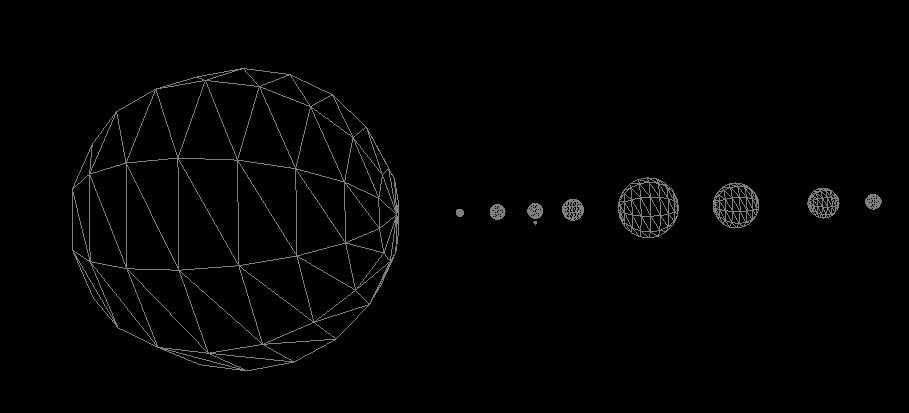
\includegraphics[width=12cm,height=6cm]{capa}
\end{figure}
\newpage

\begin{abstract}
A \textbf{Computação Gráfica}, uma das muitas áreas da informática, assume um papel fulcral em interações homem-máquina e na visualização de dados. O seu espectro de aplicações varia desde geração de imagens e animações até a simulação do mundo real. \par
	O presente relatório refere-se às diferentes fases de entrega da componente prática da Unidade Curricular de \textbf{Computação Gráfica} enquadrada no curso de \textit{Ciências da Computação} da \textit{Universidade do Minho}. 
\end{abstract}
\newpage


\tableofcontents{}
\newpage

%-------------------------------------------------
%		Introducao
%-------------------------------------------------


\section{Introdução}
Na primeira fase, foram desenvolvidas duas aplicações. Um \textbf{Gerador} de modelos, que aceite argumentos a partir do terminal, com a função de gerar os pontos de uma primitiva gráfica desejada pelo utilizador, imprimindo estes para um ficheiro. E a última, um \textbf{Motor} que interpreta os pontos gerados anteriormente de acordo com um ficheiro de configuração dado. 
Com base nos tópicos enunciados e ferramentas exploradas nas aulas implementamos o \textbf{Gerador} e o \textbf{Motor} na linguagem \textbf{C++}. Em particular esta última faz uso de biblioteca \textbf{TinyXML2} para que a leitura dos documentos que lhe são dados com input seja feita de forma simples e consistente. E por fim,  utilizamos a API fornecida pelo \textbf{OpenGl} para dar vida aos nossos modelos.\\
Na segunda, adicionamos features ao parser de ficheiros de configuração de \textbf{scenes}, nomeadamente, o reconhecimento de \textbf{scenes} dispostas hierarquicamente usando transformações geométricas (translações, rotações e de escala).//
Na terceira fase, \textbf{gerador} passa a usar patches de \textbf{ Bezier}, melhoramos as transformações do \textbf{motor} com curvas de \textbf{Catmull-Rom} e os modelos passam a ser desenhados com \textbf{VBO’s}.
E na última fase, implementamos texturas e diferentes modos de iluminação.

\newpage

\section{Primeira Fase}

\subsection{Gerador}
O nosso \textbf{Gerador} é um pequeno programa em \textbf{C++}, cuja implementação é disponibilizada em anexo, que depois de compilado, o correspondente executável escreve para um ficheiro (um por linha) os vértices da primitiva gráfica desejada  como iremos ilustrar nas seguintes secções.


\subsubsection{Caixa}
Para geração desta primitiva o utilizador deverá invocar a aplicação a com o nome do executável seguido dos comprimentos dos lados de um paraleloipipedo no eixos com X’s, Y’s e Z’s respetivamente e por fim o nome do ficheiro destino. A sintaxe é demonstrada no exemplo abaixo:

\begin{commandline}
    \begin{verbatim}
        $ g++ -o gerador gen.cpp
        $ ./gerador caixa 3 4 5 osmeusvertices
        $ ls
        $ gen.cpp            gerador            osmeusvertices.txt
    \end{verbatim}
\end{commandline}

\begin{figure}[H]
	\centering
	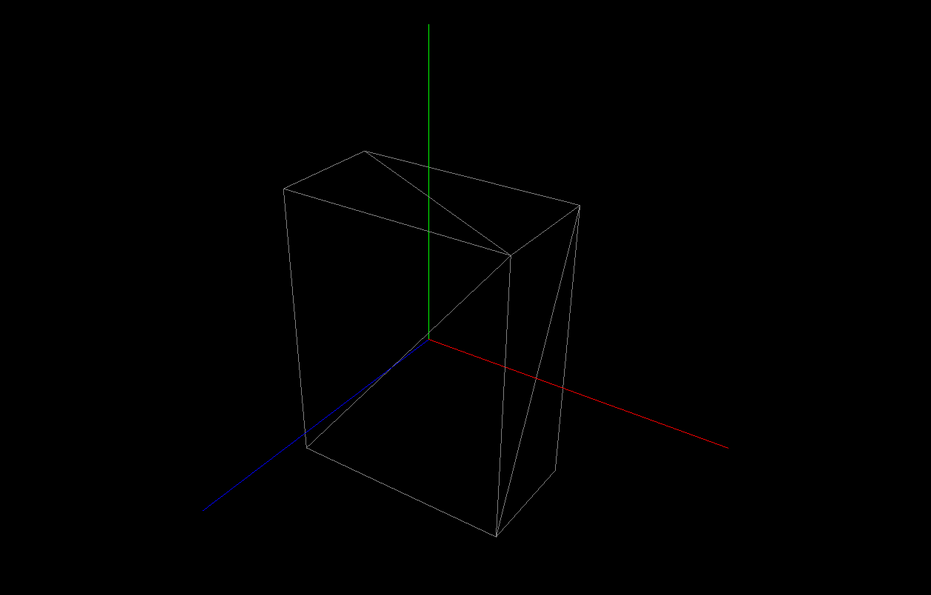
\includegraphics[width=4cm,height=4cm]{caixa}
	\caption{Caixa}
\end{figure}

\begin{warn}[Notice:]
Todas as faces são desenhadas com dois triângulos apontados para o exterior pela norma da mão direita mencionada nas aulas. Um zoom excessivo, ou a escolha de dimensões superiores à distância da câmara à origem(onde este é centrado)  pode levar ao aparente desaparecimento do modelo.
\end{warn}

\subsubsection{Cone}
O \textbf{Cone} recebe como argumentos o raio da base, a sua altura, o número de slices e stacks. \\
A construção deste começa por fixar um uma \textit{slice} calculando os vértices da base correspondente, de seguida todas as \textit{stacks} relativas, sendo o última stack - a do bico - um caso especial. \\
O algoritmo usa noções como semelhança de triângulos para cálculo dos sucessivos raios das circuferências formadas pelas \textit{stacks}.\\

\begin{info}
	Apresentamos o significado das variáveis usadas no programa que gera os pontos do \textbf{Cone}: 
	\begin{itemize}
		\item[] \textit{stkd} - diferença entre stacks consecutivas
		\item[] \textit{slcd} - diferença entre slices consecutivas
		\item[] \textit{raiod} - diferença entre o raio de duas stacks consecutivas
		\item[] \textit{stk} - stack atual 
		\item[] \textit{slc} - slice atual
		\item[] \textit{nslc} - próxima slice
		\item[] \textit{nstk} - próxima stack
		\item[] \textit{nr} - próximo raio
		\item[] \textit{r} - raio atual
	\end{itemize}
\end{info}

\begin{figure}[H]
	\centering
	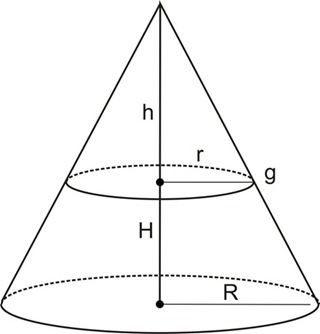
\includegraphics[width=4cm,height=4cm]{conesemelhante}
	\caption{Semelhança de triângulos num cone}
\end{figure}

Apresentamos algumas imagens que ilustram a criação do cone. \\

\begin{figure}[H]
	\centering
	\subfloat[2 stacks]{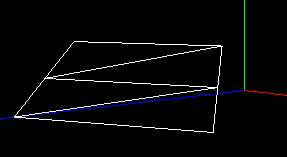
\includegraphics[width=3cm,height=3cm]{2stk}}
	\hspace{2cm}
	\subfloat[4 stacks]{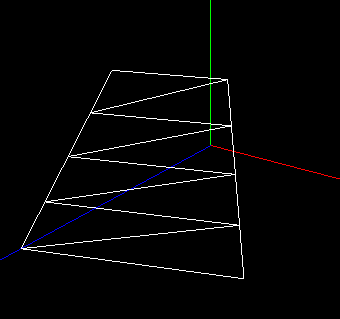
\includegraphics[width=3cm,height=3cm]{4stk}}
	\caption{Progessão das stacks do cone}
\end{figure}

\begin{figure}[H]
	\centering
	\subfloat[1 slice]{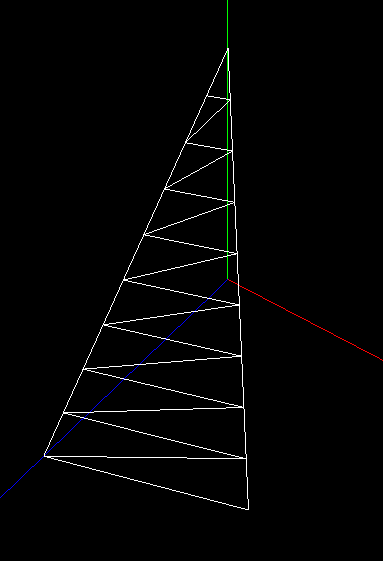
\includegraphics[width=3cm,height=3cm]{1slc}}
	\hspace{2cm}
	\subfloat[2 slices]{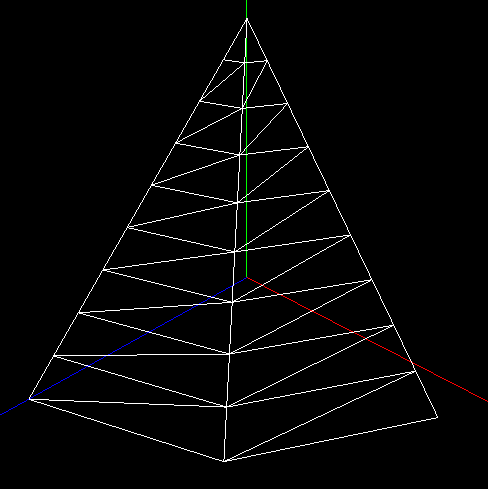
\includegraphics[width=3cm,height=3cm]{2slc}}
	\caption{Progessão das slices do cone}
\end{figure}

Finalmente obtemos:

\begin{figure}[H]
	\centering
	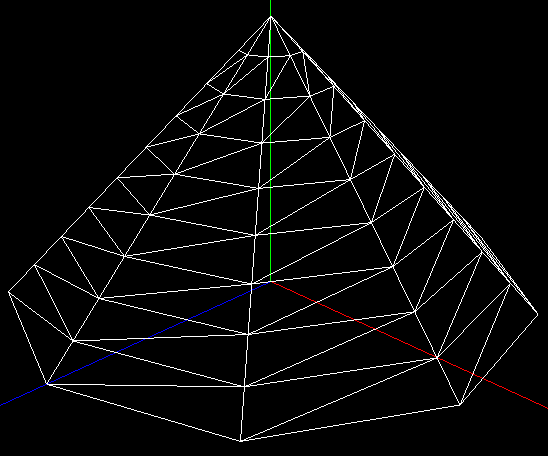
\includegraphics[width=4cm,height=4cm]{cone}
	\caption{Cone}
\end{figure}

\subsubsection{Esfera}
A \textbf{Esfera} recebe como argumentos o seu raio, o número de slices e stacks.
A sua construção usa coordenadas esféricas usando o raio dado como argumentos e manipulando 2 ângulos \textit{Alfa} e \textit{Beta}. \textit{Alfa} é dado por: \\
\[ alfa = \frac{2\times \Pi}{slices} \]
Este nos programas é usado juntamente com o raio para calcular os pontos de \textit{slices} consecutivas. De seguida \textit{beta} é dado por:\\
\[ beta = \frac{\Pi \div 2}{stacks}\] \\
Este desenpenha uma função igual ao anterior considerando \textit{stacks}.\\


\begin{figure}[H]
	\centering
	\subfloat[4 stacks]{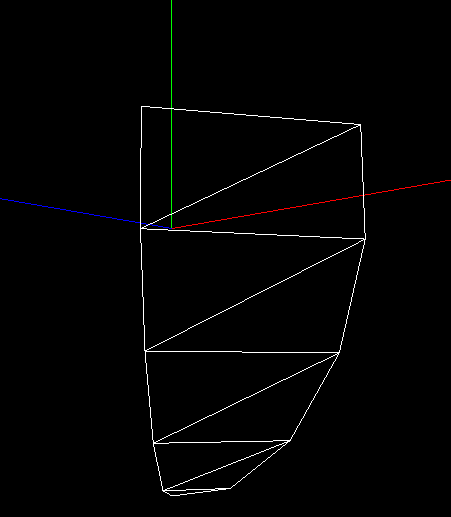
\includegraphics[width=3cm,height=3cm]{4estk}}
	\hspace{2cm}
	\subfloat[8 stacks]{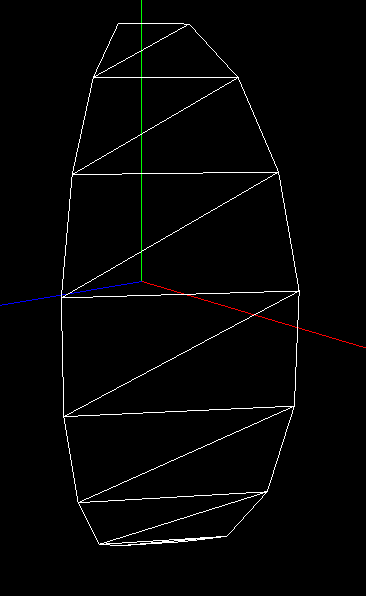
\includegraphics[width=3cm,height=3cm]{8estk}}
	\caption{Progessão das stacks da esfera}
\end{figure}

\begin{figure}[H]
	\centering
	\subfloat[1 slice]{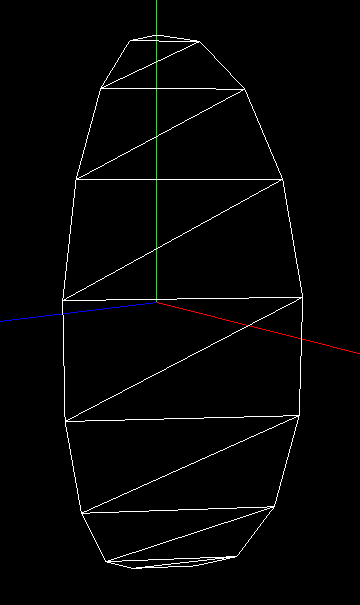
\includegraphics[width=3cm,height=3cm]{1eslc}}
	\hspace{2cm}
	\subfloat[2 slices]{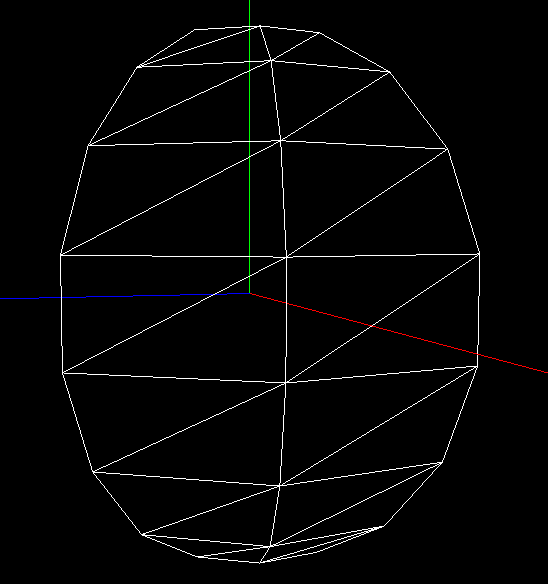
\includegraphics[width=3cm,height=3cm]{2eslc}}
	\caption{Progessão das slices da esfera}
\end{figure}

\begin{figure}[H]
	\centering
	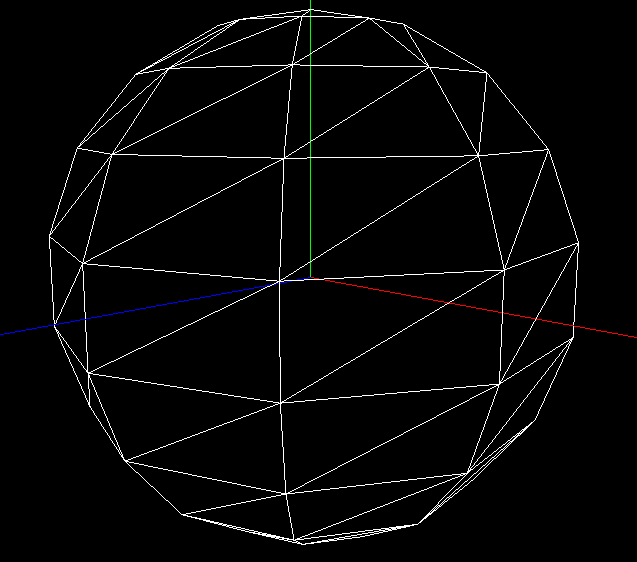
\includegraphics[width=4cm,height=4cm]{esfera}
	\caption{Esfera}
\end{figure}

\subsubsection{Plano}
O requisito estabelecido no guião do trabalho veio em muito simplificar a representação do plano XZ ao ponto de para a sua computação seja apenas necessário um único argumento que representa o tamanho da porção visível desejada.  

\begin{commandline}
    \begin{verbatim}
        $ g++ -o gerador gen.cpp
        $ ./gerador plano 5 pontos
        $ ls
        $ gen.cpp            gerador            pontos.txt
    \end{verbatim}
\end{commandline}

\begin{figure}[H]
	\centering
	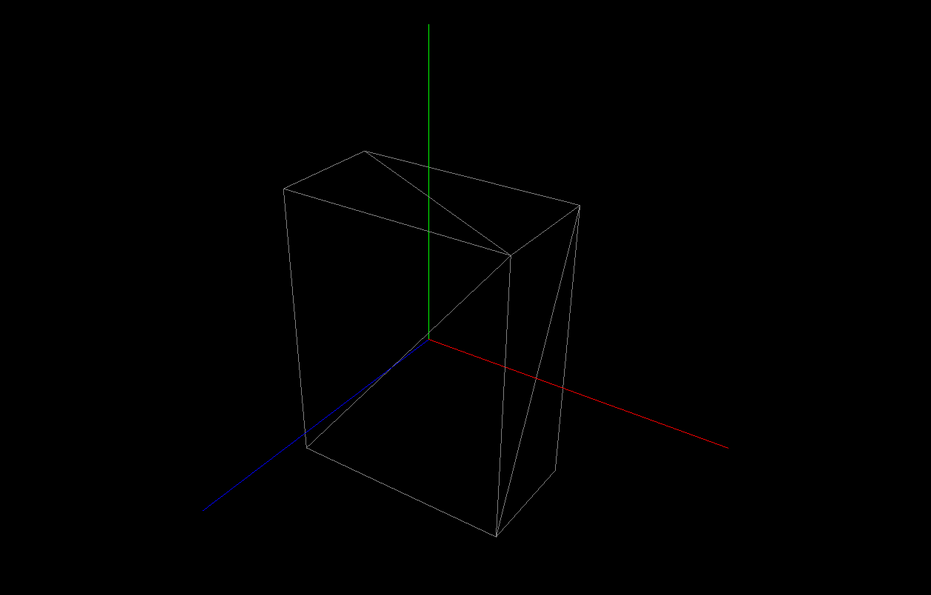
\includegraphics[width=4cm,height=4cm]{caixa}
	\caption{Caixa}
\end{figure}

\begin{warn}[Notice:]
Os planos são infinitos a referência ao tamanho é feita apenas para facilitar a observação do mesmo.
São desenhados 4 triângulos, em vez de dois, para que esta primitiva seja visível de todas as perspectivas.
\end{warn}

\newpage
\subsection{Motor}
O motor é a parte do nosso trabalho que faz o linking de todas as outras partes que foram realizadas. O motor, lê um ficheiro xml (conf.xml). Este ficheiro contém uma estrutura bastante simples, dividida em scenes.

% Contents do ficheiro conf.xml
\begin{file}[conf.xml]
	\begin{lstlisting}[language=XML]
	<scene>
		<model file="esfera.txt" />
		<model file="cone.txt" />
		<model file="caixa.txt" />
	</scene>
	\end{lstlisting}
	\end{file}

Cada ficheiro que está referenciado nas tags \textbf{<model>} é um ficheiro de texto criado pelo nosso gerador e contém todos os pontos das figuras que queremos representar.
Como o motor lê os ficheiros de pontos a partir dum ficheiro \textbf{XML} utilizamos um parser xml para \textbf{C++} chamado \textbf{tinyxml-2}.

\begin{file}[main.cpp]
	\begin{lstlisting}[language=C++]
...
tinyxml2::XMLDocument doc;

doc.LoadFile("./conf.xml");

tinyxml2::XMLNode *scene = doc.FirstChild();
		
tinyxml2::XMLElement* model;

while(scene) {
	for(model = scene->FirstChildElement();
	model != NULL; 
	model = model->NextSiblingElement()) {
		const char * file;
		file = model->Attribute("file");
		guardaPontos(file);
	}
	scene = scene->NextSiblingElement();
}
...

	\end{lstlisting}
\end{file}

Com este snippet de código, criamos um objeto do tipo XMLDocument. De seguida, com a função \textbf{LoadFile}, abrimos o ficheiro de configuração \textbf{conf.xml}, e começamos a manipular o seu conteúdo.
Criamos um objeto do tipo \textbf{XMLNode} e associamos-lhe a primeira \textbf{tag} do ficheiro conf.xml que é a raiz da estrutura do nosso ficheiro.
No ciclo while, percorremos todos o ChildElements de scene, que são as tags que guardam os nossos ficheiros das figuras.
Cada ficheiro de figura tirado dos \textbf{models} é passado à função \textbf{guardaPontos}, que será explicada de seguida.

\begin{file}[main.cpp]
	\begin{lstlisting}[language=C++]
...
struct Pontos {
    float a;
    float b;
    float c;
};

std::vector<Pontos> pontos;

void guardaPontos(std::string ficheiro) {
	std::ifstream file;
	std::string s = "./";
	s.append(ficheiro.c_str());
	file.open(s.c_str());
	float a,b,c;
	while(file >> a >> b >> c) {
		Pontos aux;
		aux.a = a;
		aux.b = b;
		aux.c = c;
		pontos.push_back(aux);
	}
}
...
	\end{lstlisting}
\end{file}

Criamos uma estrutura \textbf{Pontos} que tem como campos 3 \textit{floats}, que servem para registar as coordenadas destes. De seguida usamos um vector que utiliza a estrutura enunciada para os guardar.
À função \textbf{guardaPontos} são passados nomes de ficheiros. A função abre os ficheiros e lê pontos linha a linha, guardando cada coordenada \textit{x, y e z} num \textbf{Ponto} e de seguida inserindo-o no vector.

\begin{info} 
	A instrução:
	\begin{lstlisting}[language=C++]
		file >> a >> b >> c
	\end{lstlisting}
	associa a cada uma das variaveis \textit{a, b} e \textit{c}, as coordenadas da linha que está a ser lida em cada iteração do ciclo.
\end{info}

Por ultimo temos a função \textbf{printPontos}:

\begin{file}[main.cpp]
	\begin{lstlisting}[language=C++]
...
void printPontos(std::vector<Pontos> pontos) {
  for(int i = 0; i < pontos.size(); i++) {
		glVertex3f(pontos[i].a,
			pontos[i].b, 
			pontos[i].c);
	}
}
...
	\end{lstlisting}
\end{file}

Esta função é chamada na \text{renderScene} e geras todos os pontos percorrendo o vector.

\newpage

\section{Segunda Fase}
Após ponderarmos o enunciado, o grupo, decidiu implementar uma classe, em \textbf{C++}, inspirada numa estrutura de dados largamente conhecida na área, denominada por \textbf{Scene Graph}.\\
A origens desta estrutura de dados remonta aos primórdios dos primeiros jogos de vídeo sobre simulação de voo mas actualmente é vulgarmente incluída qualquer aplicação que lide com \textbf{Graphic Rendering}.\\
Esta estrutura de dados foi revolucionária pelo facto de reduzir drasticamente a memória necessária em cálculos sistemáticos sobre o mundo que está a tentar representar. Os cálculos passaram a ser feitos \textbf{in place} na estrutura dispensando na totalidade a necessidade de memória auxiliar. 

\subsection{A classe Scene Graph}
Apesar de disponibilizarmos a implementação em anexo iremos contemplar alguns pormenores neste capítulo.\\
Face a como os ficheiros \textbf{XML} são organizados via uma \textit{árvore} - \textit{DOM Tree} - implementamos uma classe que usa os princípios de essa mesma estrutura para guardar os dados de tudo o que é exposto na cena.\\
Por exemplo se quiséssemos desenhar um cavalo e o seu cavaleiro, não de maneira independente, mas como se o cavalo fosse uma extensão do seu cavaleiro. O \textbf{Scene Graph} correspondente teria no nodo \textbf{Cavalo} “pendurado” no nodo \textbf{Cavaleiro}.\\
Cada nodo, é um \textbf{Group} e nele guardamos as transformações geométricas que a ela lhe dizem respeito assim como um vector de pontos do \textbf{model} que queremos desenhar, e por fim, um array de outros \textbf{Scene Graphs} que representam o próximo nível de descendentes.\\

\begin{file}[main.cpp]
    \begin{lstlisting}[language=C++]

class SceneGraph {
    
    array<float, 3> scale;
    array<float, 3> trans;
    array<float, 4> rot;
    vector<vector<Ponto>> modelos;
    vector<SceneGraph> filhos;

}

    \end{lstlisting}
\end{file}

Estamos então perante a definição de uma árvore de \textbf{Scene Graphs}. Para facilitar a visualização deste conceito dispomos o seguinte exemplo.

\begin{figure}[H]
    \centering
    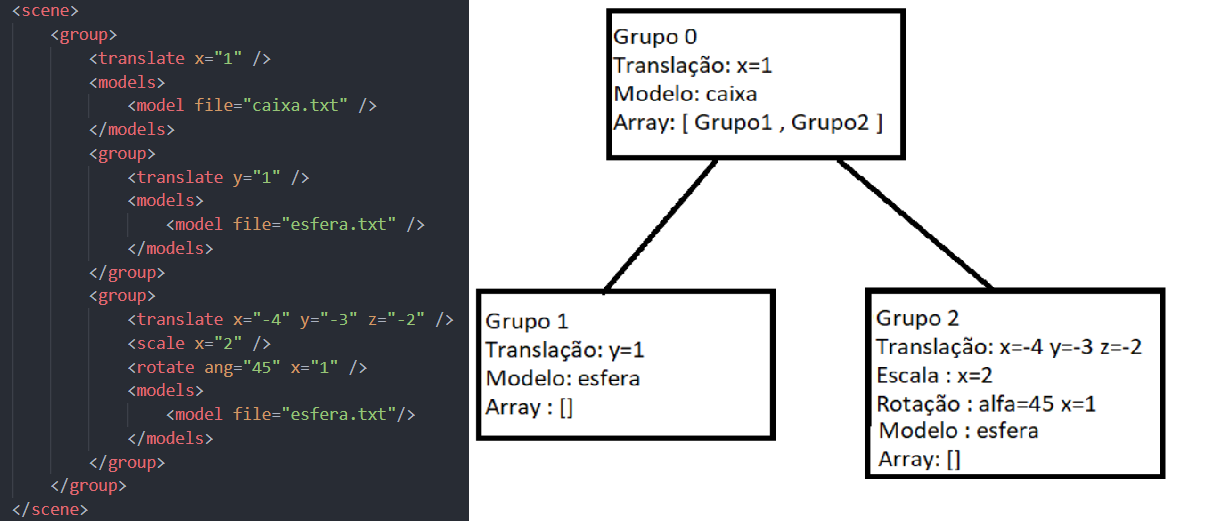
\includegraphics[width=16cm,height=6cm]{exemplo}
\end{figure}

\begin{info}
    \begin{itemize}
        \item Todos os nodos filhos herdam as transformações dos pais.
        \item Cada nodo pode ter um qualquer número de filhos, mas apenas um pai, i.e., não existe herança múltipla.
        \item Da travessia desde a raiz, até a uma folha, resultam todas as dependências que um certo objecto tem na \textbf{scene} em questão.
    \end{itemize}
\end{info}

Fixada a estrutura e comportamento do classe. Basta, agora, expor o algoritmo de travessia que é efectuada quando a nossa modesta aplicação lê um ficheiro de configuração. O resto da \textbf{API} é disponibilizada em anexo.

\begin{file}[main.cpp]
    \begin{lstlisting}[language=C++]
void SceneGraph::draw() const {

	glPushMatrix();

	glScalef(scale[0], scale[1], scale[2]);
	glRotatef(rot[0], rot[1], rot[2], rot[3]);
	glTranslatef(trans[0], trans[1], trans[2]);
	
	glBegin(GL_TRIANGLES);
	
	for( vector<Pontos> const &pnts : 
		this->modelos ) {	
		for( Pontos const &p : pnts ) {
        		glVertex3f(p.a, p.b, p.c);
    		}
	}

	glEnd();

	for( SceneGraph const &tmp : 
		this->filhos ) {
		tmp.draw();
	}

	glPopMatrix();

}   
    \end{lstlisting}
\end{file}

\begin{info}
Com base nos conteúdos abordados nas aulas teóricas decidimos adotar a convenção de ordenar as transformações geométricas \textbf{glRotatef()},\textbf{glTranslatef()} e \textbf{glSclasef()} pela sequência exposta no código acima.
\end{info}

\newpage
\subsection{Motor}
De maneira semelhante à primeira fase, o motor continua a fazer leituras de um ficheiro xml (conf.xml). Por outro lado, este ficheiro apresenta uma complexidade superior ao anterior, contendo groups, models e ainda tags de translação (\textbf{<translate>}), rotação (\textbf{<rotate>}) e mudança de escala (\textbf{<scale>}).

% Contents do ficheiro conf.xml
\begin{file}[conf.xml]
	\begin{lstlisting}[language=XML]
<scene>
    <group>
        <translate x="1" />
        <models>
            <model file="caixa.txt" />
        </models>
        <group>
            <translate y="1" />
            <models>
                <model file="esfera.txt" />
            </models>
        </group>
        <group>
            <translate x="-4" y="-3" z="-2" />
            <scale x="2" />
            <rotate ang="45" x="1" />
            <models>
                <model file="esfera.txt"/>
            </models>
        </group>
    </group>
</scene>
	\end{lstlisting}
	\end{file}

Cada ficheiro que está referenciado nas tags \textbf{<model>} é um ficheiro de texto criado pelo nosso gerador e contém todos os pontos das figuras que queremos representar.
Como o motor lê os ficheiros de pontos a partir dum ficheiro \textbf{XML} utilizamos um parser xml para \textbf{C++} chamado \textbf{tinyxml-2}.

\begin{file}[main.cpp]
	\begin{lstlisting}[language=C++]
...
tinyxml2::XMLDocument doc;
//new file
doc.LoadFile("./conf.xml");
tinyxml2::XMLNode *scene = doc.FirstChild();
if (scene == nullptr) perror("Erro de Leitura.\n");

s_gg = doGroup(scene->FirstChildElement("group"));
...
	\end{lstlisting}
\end{file}

Com este snippet de código, criamos um objeto do tipo XMLDocument. De seguida, com a função \textbf{LoadFile}, abrimos o ficheiro de configuração \textbf{conf.xml}, Criamos um objeto do tipo \textbf{XMLNode} e associamos-lhe a primeira \textbf{tag} do ficheiro conf.xml que é a raiz da estrutura do nosso ficheiro.
Através da função doGroup, começamos a manipular o seu conteúdo.

\begin{file}[engine.cpp]
	\begin{lstlisting}[language=C++]
SceneGraph doGroup(tinyxml2::XMLElement* group) {
    SceneGraph s_g;
    tinyxml2::XMLElement* novo = 
	group->FirstChildElement();
    for(novo; novo != NULL; 
	novo = novo->NextSiblingElement()) {
        //printf("%s\n", novo->Name());
        if(!strcmp(novo->Name(), "group")) {
            s_g.addFilho(doGroup(novo));
        } else if(!strcmp(novo->Name(), "models")) {
            s_g.setModelo(doModels(novo));
        } else if(!strcmp(novo->Name(), 
		"translate")) {
            s_g.setTrans(doTranslate(novo));
        } else if(!strcmp(novo->Name(), "rotate")) {
            s_g.setRot(doRotate(novo));
        } else if(!strcmp(novo->Name(), "scale")) {
            s_g.setScale(doScale(novo));
        } else {
            perror("Formato XML Incorreto.\n");
        }
    }
return s_g;
}
	\end{lstlisting}
\end{file}

No ciclo \textit{for}, percorremos todos o ChildElements da group, que são as tags que guardam os nossos ficheiros das figuras.
Dentro de cada tag \textbf{group} pode haver outra tag \textbf{group}, ativando a recursão da função doGroup. Mas, há outras tags que podem aparecer, tais como \textbf{models} \textbf{<translate>}, \textbf{<rotate>} e \textbf{<scale>}.
Caso a tag lida seja \textbf{<translate>}, a função doGroup evoca a função doTranslate:

\begin{file}[engine.cpp]
	\begin{lstlisting}[language=C++]
array<float,3> doTranslate(
	tinyxml2::XMLElement* translate) {

    array<float, 3> trans;
    
    const char * x;
    const char * y;
    const char * z;
    x = translate->Attribute("x");
    y = translate->Attribute("y");
    z = translate->Attribute("z");
    
    x == nullptr ? trans[0] = 0 : trans[0] = atof(x);
    y == nullptr ? trans[1] = 0 : trans[1] = atof(y);
    z == nullptr ? trans[2] = 0 : trans[2] = atof(z);
    
    return trans;
}
	\end{lstlisting}
\end{file}

Caso a tag lida seja \textbf{<rotate>}, a função doGroup evoca a função doRotate:

\begin{file}[engine.cpp]
	\begin{lstlisting}[language=C++]
array<float,4> doRotate(tinyxml2::XMLElement* rotate) {

    array<float,4> rot;

    const char * x;
    const char * y;
    const char * z;
    const char * ang;
    x = rotate->Attribute("x");
    y = rotate->Attribute("y");
    z = rotate->Attribute("z");
    ang = rotate->Attribute("angle");

    ang == nullptr ? rot[0] = 0 : rot[0] = atoi(ang);
    x == nullptr ? rot[1] = 0 : rot[1] = atof(x);
    y == nullptr ? rot[2] = 0 : rot[2] = atof(y);
    z == nullptr ? rot[3] = 0 : rot[3] = atof(z);

    return rot;	
}
	\end{lstlisting}
\end{file}

Caso a tag lida seja \textbf{<scale>}, a função doGroup evoca a função doScale:

\begin{file}[engine.cpp]
	\begin{lstlisting}[language=C++]
array<float,3> doScale(tinyxml2::XMLElement* scale) {

    array<float,3> sca;
    
    const char * x;
    const char * y;
    const char * z;
    
    x = scale->Attribute("x");
    y = scale->Attribute("y");
    z = scale->Attribute("z");
    
    x == nullptr ? sca[0] = 1 : sca[0] = atof(x);
    y == nullptr ? sca[1] = 1 : sca[1] = atof(y);
    z == nullptr ? sca[2] = 1 : sca[2] = atof(z);
    
    return sca;
}
	\end{lstlisting}
\end{file}

Qualquer uma destas 3 funções, retorna um array com os argumentos que serão passados às funções Glut que executarão as transformações: a função doTranslate, retorna um array com 3 argumentos para a função \textbf{glTranslate}, a função doRotate, retorna um array com 4 argumentos para a função \textbf{glRotate} e a função doScale, retorna um array com 3 argumentos para a função \textbf{glScale}.

\par Por outro lado, ainda pode aparecer uma tag \textbf{<models>}, ou seja é chamada a função doModels que significa que, dentro dessas tags, vai haver uma tag \textbf{<model file= "nome do ficheiro.txt">}, ficheiro este que tem todos os pontos gerados pelo gerador. 

\begin{file}[engine.cpp]
	\begin{lstlisting}[language=C++]
std::vector<std::vector<Pontos>> 
	doModels(tinyxml2::XMLElement* models) {
    std::vector<std::vector<Pontos>> pPontos;
    tinyxml2::XMLElement* novo = 
	models->FirstChildElement();
    for(novo; novo != NULL; 
	novo = novo->NextSiblingElement()) {
        const char * file;
        file = novo->Attribute("file");
        pPontos.push_back(guardaPontos(file));
    }
    return pPontos;
}
	\end{lstlisting}
\end{file}
	
A função doModels chama a função \textbf{guardaPontos} que, usando a estrutura \textbf{Pontos}, regista as coordenadas de cada ponto presente no ficheiro. A estrutura tem campos 3 \textit{floats}, que servem para guardar as coordenadas dos pontos. De seguida usamos um vector que utiliza a estrutura enunciada para os guardar.
A função abre os ficheiros e lê pontos linha a linha, guardando cada coordenada \textit{x, y e z} num \textbf{Ponto} e de seguida inserindo-o no vector.

\begin{file}[engine.cpp]
	\begin{lstlisting}[language=C++]
...
struct Pontos {
    float a;
    float b;
    float c;
};

std::vector<Pontos> pontos;

void guardaPontos(std::string ficheiro) {
	std::ifstream file;
	std::string s = "./";
	s.append(ficheiro.c_str());
	file.open(s.c_str());
	float a,b,c;
	while(file >> a >> b >> c) {
		Pontos aux;
		aux.a = a;
		aux.b = b;
		aux.c = c;
		pontos.push_back(aux);
	}
}
...
	\end{lstlisting}
\end{file}

Este array de pontos que a guardaPontos retorna, preenche o array pPontos instanciado na doModels, que por sua vez é retornado por esta função. Na função doGroup, uma SceneGraph é passada como objeto aos Setters definidos na estrutura SceneGraph, que chamam as funções acima faladas que, retornandos os arrays de argumentos e os pontos das figuras, fazem uma atualização da estrutura, que na \textbf{main.cpp} é passada à renderScene.
\newpage

\section{Terceira Fase}

Os requisitos para esta fase são:
\begin{itemize}
	\item O gerador tem agora de ser capaz de criar um novo modelo baseado em \textbf{patches} de \textbf{Bezier};
	\item O motor terá que enriquecer a sua definicão de duas transformações geométricas. As \textit{translações} poderam agora receber um conjunto de pontos (com um mínimo de 4 elementos), sendo estes os pontos de controlo de uma curva de \textbf{Catmull-Rom}, e um tempo (em segundos) para percorrer a curva. O objetivo é realizar animações baseadas nestas curvas. As \textit{rotações} podem agora receber um tempo (novamente em segundos) em vez de um ângulo, este server para descrever o tempo para se realizar uma rotação de 360º. Estas também com o objetico de animar objetos no sistema;
	\item Por fim, os modelos têm agora de ser desenhados usando \textbf{VBO}'s.
\end{itemize}

Os requisitos levaram a atualização de alguns conceitos e a criação de novos. Descrevemos todas estas mudanças nos capítulos que se seguem.

\subsection{Link para um streamable com a demonstrar animação}
LINK - \url{https://streamable.com/k2906}

\subsection{Modificações à classe SceneGraph}

A classe \textbf{SceneGraph}, introduzida na \textbf{Etapa 2} sofreu alguma restruturação. Os \textit{arrays} que eram usados para guardar as várias \textit{tranformações geométricas} passaram agora a ser classes com o seu próprio comportamento. Foram criados dois novo objetos \textbf{TranslacaoC} e \textbf{RotacaoT} para lidar com os novos requisitos referentes às translações e rotações. O objeto \textbf{SceneGraph} passou a ter uma variável de instância \textit{vbo}, esta, como o nome indica, é usada para desenhar os modelos usando \textbf{VBO}'s. As mundanças são apresentadas em maior detalhe nos capítulos seguintes.

\subsubsection{Redefinição de Conceitos}
\subsubsection*{Arrays}
Como mencionado acima os \textbf{arrays} foram convertidos para classes. Esta mudança veio a propósito de tornar mais fácil o trabalho a desenvolver com esta, face ao aumento em número das suas variáveis de instância e com isto, a sua complexidade. Estas apresentam a mesma funcionalidade da etapa anterior. \\
O \textit{array} que codificava uma rotação simples passou a ser definido por:
\begin{file}[conversao.cpp]
        \begin{lstlisting}[language=C++]
array<float, 4> rot
		
		//para

// RotacaoV = Rotacao Vetorial
class RotacaoV {

	array<float, 4> rot;

	public:
		RotacaoV();
		void setRot( array<float, 4> );
		void aplica();
};
	\end{lstlisting}
\end{file}

Os métodos a que esta responde (e de forma similar todas as outras transformações estáticas ) são um \textit{setter} para mudar o seu estado interno e a função \textit{aplica} que será usada na altura de desenhar para aplicar a transformação aos modelos.
As restantes classes mais simples apresentam uma conversão similar, pelo que escusámos de as apresentar todas aqui.

\subsubsection*{Modelos}

Os modelos guardados passaram agora a ser uma \textit{vector} de \textit{float}'s em vez de um da estrutra \textit{Pontos} para facilitar a sua impressão via \textbf{VBO}'s.  

\begin{file}[conversao.cpp]
        \begin{lstlisting}[language=C++]
...
vector<Pontos> modelos;
...		
		//para
...
vector<float> modelos;
...
	\end{lstlisting}
\end{file}

A existência de métodos como \textit{data}, \textit{size} e ainda \textit{insert} facilitam a transição para \textbf{VBO}'s.

\subsubsection*{Método draw}

O método encarregue de desenhar os modelos sofreu como de esperar algumas mudanças.

\begin{file}[drawantigo.cpp]
        \begin{lstlisting}[language=C++]
void SceneGraph::draw() const {

    glPushMatrix();

    glScalef(scale[0], scale[1], scale[2]);
    glRotatef(rot[0], rot[1], rot[2], rot[3]);
    glTranslatef(trans[0], trans[1], trans[2]);

    glBegin(GL_TRIANGLES);

    for( vector<Pontos> const &pnts : 
	this->modelos ) {
        for( Pontos const &p : pnts ) {
                glVertex3f(p.a, p.b, p.c);
            }
    }
    glEnd();
    for( SceneGraph const &tmp : this->filhos ) {
        tmp.draw();
    }
    glPopMatrix();
}
	\end{lstlisting}
\end{file}

Este passa agora a chamar os métodos \textit{aplica} em vez de explicitamente fazer as transformações, sendo posteriormente feito o \textit{bind} a partir da variável \textit{vbo}. Os argumentos da função \textit{VertexPointer} e \textit{glDrawArrays}. Também importante notar o \textit{booleano} usado para sinalizar quando as transformações dinãmicas têm de ser aplicadas(n vezes por segundo).

\begin{file}[drawnovo.cpp]
        \begin{lstlisting}[language=C++]
void SceneGraph::draw( bool updt ) {

    glPushMatrix();

    this->scale.aplica();
    this->rot.aplica();
    this->trans.aplica();

    this->curva.aplica( updt );
    this->eixo.aplica( updt );

    glBindBuffer(GL_ARRAY_BUFFER, this->vbo);
    glVertexPointer(3,GL_FLOAT, 0, 0);

    glDrawArrays(GL_TRIANGLES, 0, 
	this->modelos.size() / 3);

    for( SceneGraph &tmp : this->filhos ) {
        tmp.draw( updt );
    }

    glPopMatrix();

}
	\end{lstlisting}
\end{file}

\begin{info}
	De notar a ordem com que as transformações são aplicadas. As estáticas são priorizadas (mantendo a ordem da etapa anterior), sendo das dinâmicas aplicada primeiro a translação e por fim a rotação.
\end{info}

\subsubsection{Novas Funcionalidades}
Para satisfazer os requisitos, foram criadas as classes:
\begin{itemize}
	\item \textbf{TranslacaoC} - para codificar a animação a partir de uma curva de \textbf{CatmullRom};
	\item \textbf{RotacaoT} - para codificar a animação de um planeta em torno de um eixo dado um fator temporal.
\end{itemize}


Da classe \textbf{TranslacaoC}, apresentamos o seu método principal:

\begin{file}[transC.cpp]
        \begin{lstlisting}[language=C++]
void TranslacaoC::setCurva( vector<Pontos> pntCnt, 
	int tempoVolta ) {

    Pontos aux;
    float tseg = 1.0f / tempoVolta;

    if( !pntCnt.empty() ) {
        for(int i = 0; i < tempoVolta; i++) {
            getGlobalCatmullRomPoint(i * tseg, 
	    pntCnt.data(), pntCnt.size(), &aux);
            this->pntsCurva.push_back(aux);
        }
    }
}
	\end{lstlisting}
\end{file}

Que aceita um \textit{vector} de pontos de controlo da curva e o tempo para dar uma volta. Esta calcula os pontos por onde o objeto passa a cada segundo da volta, guardando-os.

De seguida, da classe \textbf{RotacaoT} apresentamos os métodos que gerem o estado interno.

\begin{file}[RotacaoT.cpp]
        \begin{lstlisting}[language=C++]
void RotacaoT::setRot( array<float, 3> axs ) {
    this->rot[1] = axs[0];
    this->rot[2] = axs[1];
    this->rot[3] = axs[2];
}

void RotacaoT::setGraus( int tempoVolta ) {
    this->rot[0] = 360.0f / tempoVolta;
    this->segundos = tempoVolta;
}
	\end{lstlisting}
\end{file}


\subsection{A classe TimedSG} 

Esta classe utiliza os objetos \textbf{SceneGraph} e \textbf{Cronometro} para conseguir trazer animações ao motor.

\begin{file}[Cronometro.cpp]
        \begin{lstlisting}[language=C++]

bool Cronometro::updateTime() {

    int aux = glutGet(GLUT_ELAPSED_TIME);

    if(aux - this->basetime >= 25) {
        this->basetime = aux;
        return true;
    }

    return false;

}
	\end{lstlisting}
\end{file}

A classe \textbf{Cronometro} apresenta apenas um método, este compara um tempo previamente registado ao tempo atual e se este for maior que um delta atualiza o seu valor interno e devolve \textit{true}, caso contrário devolve \textit{false}. 
Este boleano é usado na classe seguinte para determinar se as trasformações dinâmicas têm de movimentar os seus objetos.

\begin{file}[timedsg.cpp]
	\begin{lstlisting}
TimedSG::TimedSG() {

}

void TimedSG::setSG( SceneGraph novoSG ) {

    this->sg = novoSG;

}

void TimedSG::prep() {

    this->sg.prep();

}

void TimedSG::draw() {

    bool aux = this->tmp.updateTime();
    this->sg.draw( aux );
}
	\end{lstlisting}
\end{file}

\subsection{Atualizações ao Motor}

A nível do parse do ficheiro .xml, é criado um \textbf{XMLNode} com a primeira tag \textbf{gorup}, e passando a mesma à função \textbf{doGroup} que trata todas as tags desse groupo. O que difere da fase anterior é que as informações são passadas por objetos, sendo que vai haver uma função associada a cada tag lida, que mantém a funcionalidade registada na fase anterior. À semelhança da fase anterior, caso a tag lida seja group, é chamada a doGroup de novo de maneira recursiva.\\
Porém, nesta nova fase foi introduzida a noção de curvas e tempo. O que significa que tivemos que fazer mudanças na função doGroup para puder receber estas tags com \textbf{Atribute time}.\\

\begin{file}[engine.cpp]
    \begin{lstlisting}[language=C++]
	SceneGraph doGroup(tinyxml2::XMLElement* group) {
	    SceneGraph s_g;
	    tinyxml2::XMLElement* novo = group->FirstChildElement();
	    for(novo; novo != NULL; novo = novo->NextSiblingElement()) {
	        //printf("%s\n", novo->Name());
	        if(!strcmp(novo->Name(), "group")) {
	            s_g.addFilho(doGroup(novo));
	        } else if(!strcmp(novo->Name(), "models")) {
	            s_g.setModelo(doModels(novo));
	        } else if(!strcmp(novo->Name(), "translate")) {
	            if(novo->Attribute("time") == nullptr) {
	                s_g.setTrans(doTranslate(novo));
	            } else {
	                s_g.setCurva(doTimeTranslate(novo));
	            }
	        } else if(!strcmp(novo->Name(), "rotate")) {
	            if(novo->Attribute("time") == nullptr) {
	                s_g.setRot(doRotate(novo));
	            } else {
	                s_g.setEixo(doTimeRotate(novo));
	            }
	        } else if(!strcmp(novo->Name(), "scale")) {
	            s_g.setScale(doScale(novo));
	        } else {
	            perror("Formato XML Incorreto.\n");
	        }
	    }
	    return s_g;
	}
    \end{lstlisting}
\end{file}
As novas tags podem ser \textbf{translate time} e \textbf{rotate time} e para isso foram criadas duas novas funções: \textbf{doTimeTranslate} e \textbf{doTimeRotate} para tratar cada uma das tags, respetivamente.

\begin{file}[engine.cpp]
    \begin{lstlisting}[language=C++]
	TranslacaoC doTimeTranslate(tinyxml2::XMLElement* translate) {

	    TranslacaoC t;

	    int tempo;
	    tempo = atoi(translate->Attribute("time"));

	    std::vector<Pontos> pontos;

	    tinyxml2::XMLElement* point = translate->FirstChildElement();
	    for(point; point != NULL; point = point->NextSiblingElement()) {
	        Pontos aux;
	        aux.a = atof(point->Attribute("x"));
	        aux.b = atof(point->Attribute("y"));
	        aux.c = atof(point->Attribute("z"));
	        pontos.push_back(aux);
	    }
	    if(pontos.size() < 4) {
	        perror("Sao necessarios no minimo 4 pontos");
	    } else {
	        t.setCurva(pontos, tempo);
	    }
	    return t;
	}
    \end{lstlisting}
\end{file}

\begin{file}[engine.cpp]
    \begin{lstlisting}[language=C++]
	RotacaoT doTimeRotate(tinyxml2::XMLElement* rotate) {

	    RotacaoT rotation;

	    std::array<float, 3> xyz;

	    int tempo;

	    xyz[0] = atof(rotate->Attribute("x"));
	    xyz[1] = atof(rotate->Attribute("y"));
	    xyz[2] = atof(rotate->Attribute("z"));

	    tempo = atoi(rotate->Attribute("time"));

	    rotation.setRot(xyz);
	    rotation.setGraus(tempo);

	    return rotation;
	}
    \end{lstlisting}
\end{file}

\subsection{Atualizações ao Gerador}
Não contemplamos mudanças ao gerador nesta fase. (Bezier patches não implementadas).

\newpage
\section{Quarta fase}

\subsection{Gerador}
O \textbf{Gerador} tem de também de imprimir no ficheiro alvo, que á semelhança das fases anteriores é escolhido pelo utilizador, para cada vertice, a normal e as coordenadas no espaço textura.\\
Por uma questão de organização adoptamos a convenção na primiera linha do ficheiro consta sempre o numero vertices, seguidos das componentes das coordenadas dos vertices, depois das normais e por fim das texturas (uma por linha).\\
\subsubsection{ Calculo Normais }
As normais dos pontos de um objecto servem para que o \textbf{OpenGl} possa calcular o comportamento da luz ao longo das superficies da primitiva. Todos estes valores são armazenados na sua forma normalizada para garantir eficiencia e comportamentos "estranhos".\\

\subsubsection{ Plano } 
No caso de um plano XZ é trivialmente verdade que a normal é a mesma em todos os pontos do plano e que é igual a (0,1,0). No entanto, para que o comportamento da luz seja equivalente na frente eno verso desta primitiva, associamos a normal (0,-1,0) aos pontos do verso do plano.
\begin{figure}[H]
	\centering
	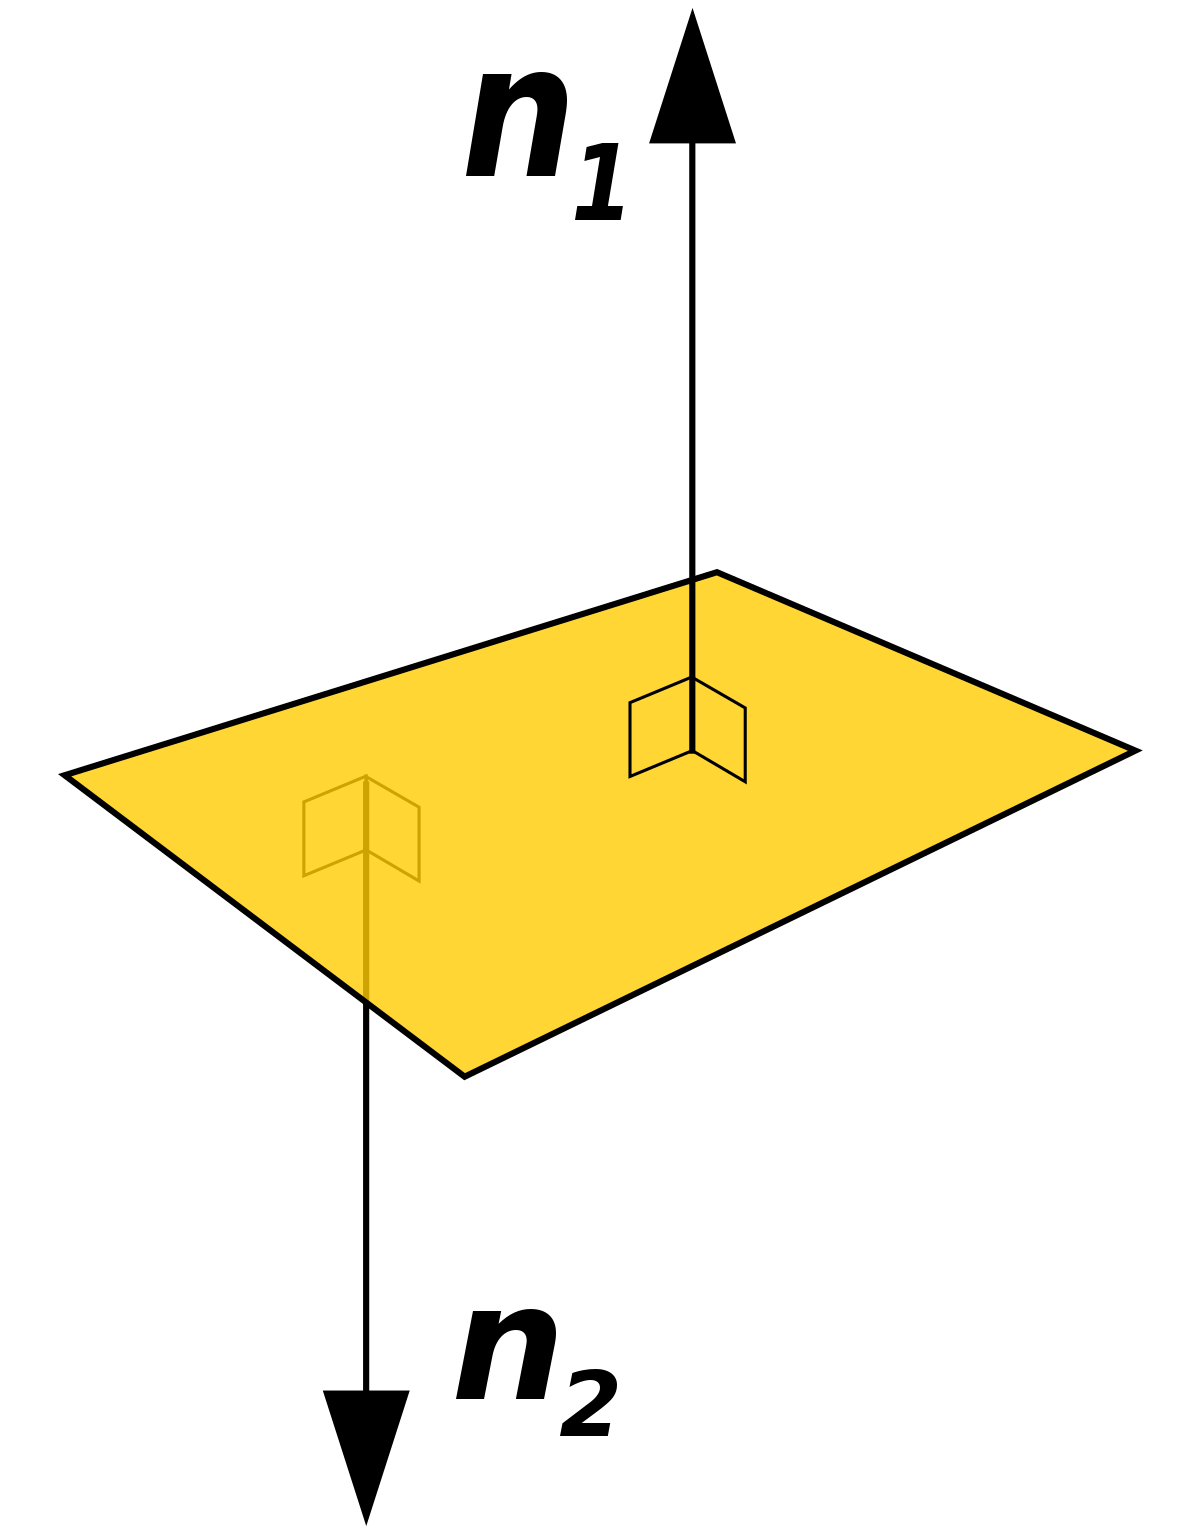
\includegraphics[width=12cm,height=6cm]{plan}
\end{figure}

\subsubsection{ Caixa }
Se subdividirmos esta primitiva nas fases que a constituem caimos no caso da primitiva anterior. De emidiato vem que para as fases paralelas a XY as normais são (0,0,1) e (0,0,-1), a XZ (0,1,0) e (0,-1,0) e por fim as YZ (1,0,0) e (-1,0,0).\\  
\begin{figure}[H]
	\centering
	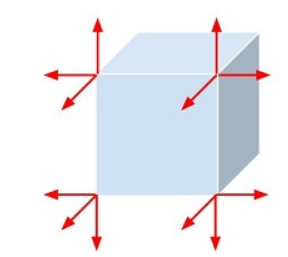
\includegraphics[width=12cm,height=6cm]{Capture}
\end{figure}

\subsubsection{ Esfera }
No caso desta primitiva, como já trabalhamos com coordenadas polares para gerar os vertices, as normais de cada ponto podem ser facilmente obtidas se considerarmos uma esfera de raio 1.  
\begin{figure}[H]
	\centering
	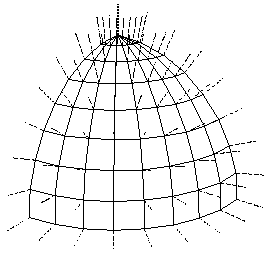
\includegraphics[width=12cm,height=6cm]{esfer}
\end{figure}

\subsubsection{ Cone }
A base do cone esta em XZ, é novamente o caso do plano, portanto, a sua normal é (0,1,0). 
\begin{figure}[H]
	\centering
	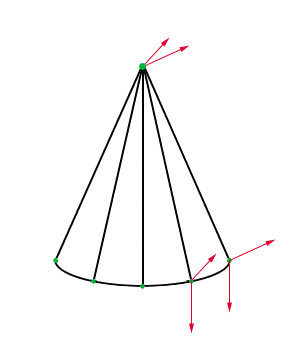
\includegraphics[width=12cm,height=6cm]{cione}
\end{figure}

\subsubsection{Mapeamento de Texturas}

\section{ Esfera }
Sejam  alpha e beta os angulos que variam, respetivamente [0..2*PI] e [-PI/2 ... PI /2], facilmente se mapeam para espaço textura (u e v ambos a variar entre 0 e 1 ) com a trnaformação u = a / (2 * PI) e v = (b / PI) + 0.5\\ 

\section{ Box }
Sejam i e j as variaveis que iteram as subdivisoes da caixa (ndivs) nos eixos XX e ZZ respetivamente, mapeamos  u =  i / ndivs e v = j / ndivs.
\subsubsection{ Plano } 
Neste caso basta mapear as extremidades do plano para a extremidade correspondente da imagem, isto é ,  canto superior direito do plano para (1,1), canto superior esquerdo do plano para (-1,1), canto inferior direito do plano para (1,-1) e o canto inferior esquerdo do plano para (-1,-1) . 
\subsubsection{ Cone } 
tambem eu gostava de saber

\section{Conclusão}
Também nos ajudou a possuir mais discernimento sobre a geometria e cálculos matemáticos por detrás de todo um esquema geométrico em 3 dimensões.\\
Durante a realização dos geradores conseguimos perceber que a propagação dos erros nos cálculos dos ângulos pode ter impacto na apresentação das figuras geométricas.\\
Apresentou-nos também mais uma oportunidade de aprender e melhorar as nossas capacidades de programação em C++, no uso de LaTex e de ficheiros XML.\\
Todas as aptidões aqui aprendidas e/ou desenvolvidas, não só a nível escolar mas como a nível de cooperação e  de trabalho de equipa. vão-nos permitir uma melhor realização de projetos futuros.\\
A realização desta fase, ajudou-nos a ganhar um conhecimento mais profundo no âmbito das curvas e superfícies de Bezier e do cálculo por detrás do algoritmo de Catmull-Rom, conhecimento sobre rotações e translações face ao tempo. À medida que vamos avançando no projeto, a complexidade do mesmo vai aumentando, o que também nos trás a oportunidade de melhorar as nossas capacidades de programação em C++, e do uso das funções das bibliotecas leccionadas nas aulas.\\
Está secção poderá ser modificada ao longo das fases de entrega.\\

\newpage


\appendix

\section{Biblioteca CatmullRomMath}
\lstinputlisting[language = C++]{../Deps/catmullmath.h}
\lstinputlisting[language = C++]{../Deps/catmullmath.cpp}
\newpage

\section{Biblioteca Cronometro}
\lstinputlisting[language = C++]{../Deps/cronometro.h}
\lstinputlisting[language = C++]{../Deps/cronometro.cpp}
\newpage

\section{Biblioteca Engine}
\lstinputlisting[language = C++]{../Deps/engine.h}
\lstinputlisting[language = C++]{../Deps/engine.cpp}
\newpage

\section{Biblioteca Escala}
\lstinputlisting[language = C++]{../Deps/escala.h}
\lstinputlisting[language = C++]{../Deps/escala.cpp}
\newpage

\section{Biblioteca RotacaoT}
\lstinputlisting[language = C++]{../Deps/rotacaoT.h}
\lstinputlisting[language = C++]{../Deps/rotacaoT.cpp}
\newpage

\section{Biblioteca RotacaoV}
\lstinputlisting[language = C++]{../Deps/rotacaoV.h}
\lstinputlisting[language = C++]{../Deps/rotacaoV.cpp}
\newpage

\section{Biblioteca SceneGraph}
\lstinputlisting[language = C++]{../Deps/sg.h}
\lstinputlisting[language = C++]{../Deps/sg.cpp}
\newpage

\section{Biblioteca TimedSG}
\lstinputlisting[language = C++]{../Deps/timedsg.h}
\lstinputlisting[language = C++]{../Deps/timedsg.cpp}
\newpage

\section{Biblioteca TranslacaoC}
\lstinputlisting[language = C++]{../Deps/translacaoC.h}
\lstinputlisting[language = C++]{../Deps/translacaoC.cpp}
\newpage

\section{Biblioteca TranslacaoV}
\lstinputlisting[language = C++]{../Deps/translacaoV.h}
\lstinputlisting[language = C++]{../Deps/translacaoV.cpp}
\newpage

\section{Código da Main}
\lstinputlisting[language=C++]{../main.cpp}
\newpage

\section{Codigo do Gerador}
\lstinputlisting[language=C++]{../gen.cpp}
\newpage

\section{XML usado para a animação}
\lstinputlisting{./conf.xml}
\end{document}
